\usepackage{extras}

\usetheme{default}
\usecolortheme{dove}

\title{Konstruktion av en autonom undsättningsrobot}
\subtitle{Kandidatprojekt i elektronik vid Linköpings universitet}
\author{Grupp 4}
\beamertemplatenavigationsymbolsempty
\date{\today}

\begin{document}

\begin{frame}
  \titlepage
\end{frame}


\begin{frame}{PigBot}
  \begin{columns}
    \begin{column}{0.5\textwidth}
      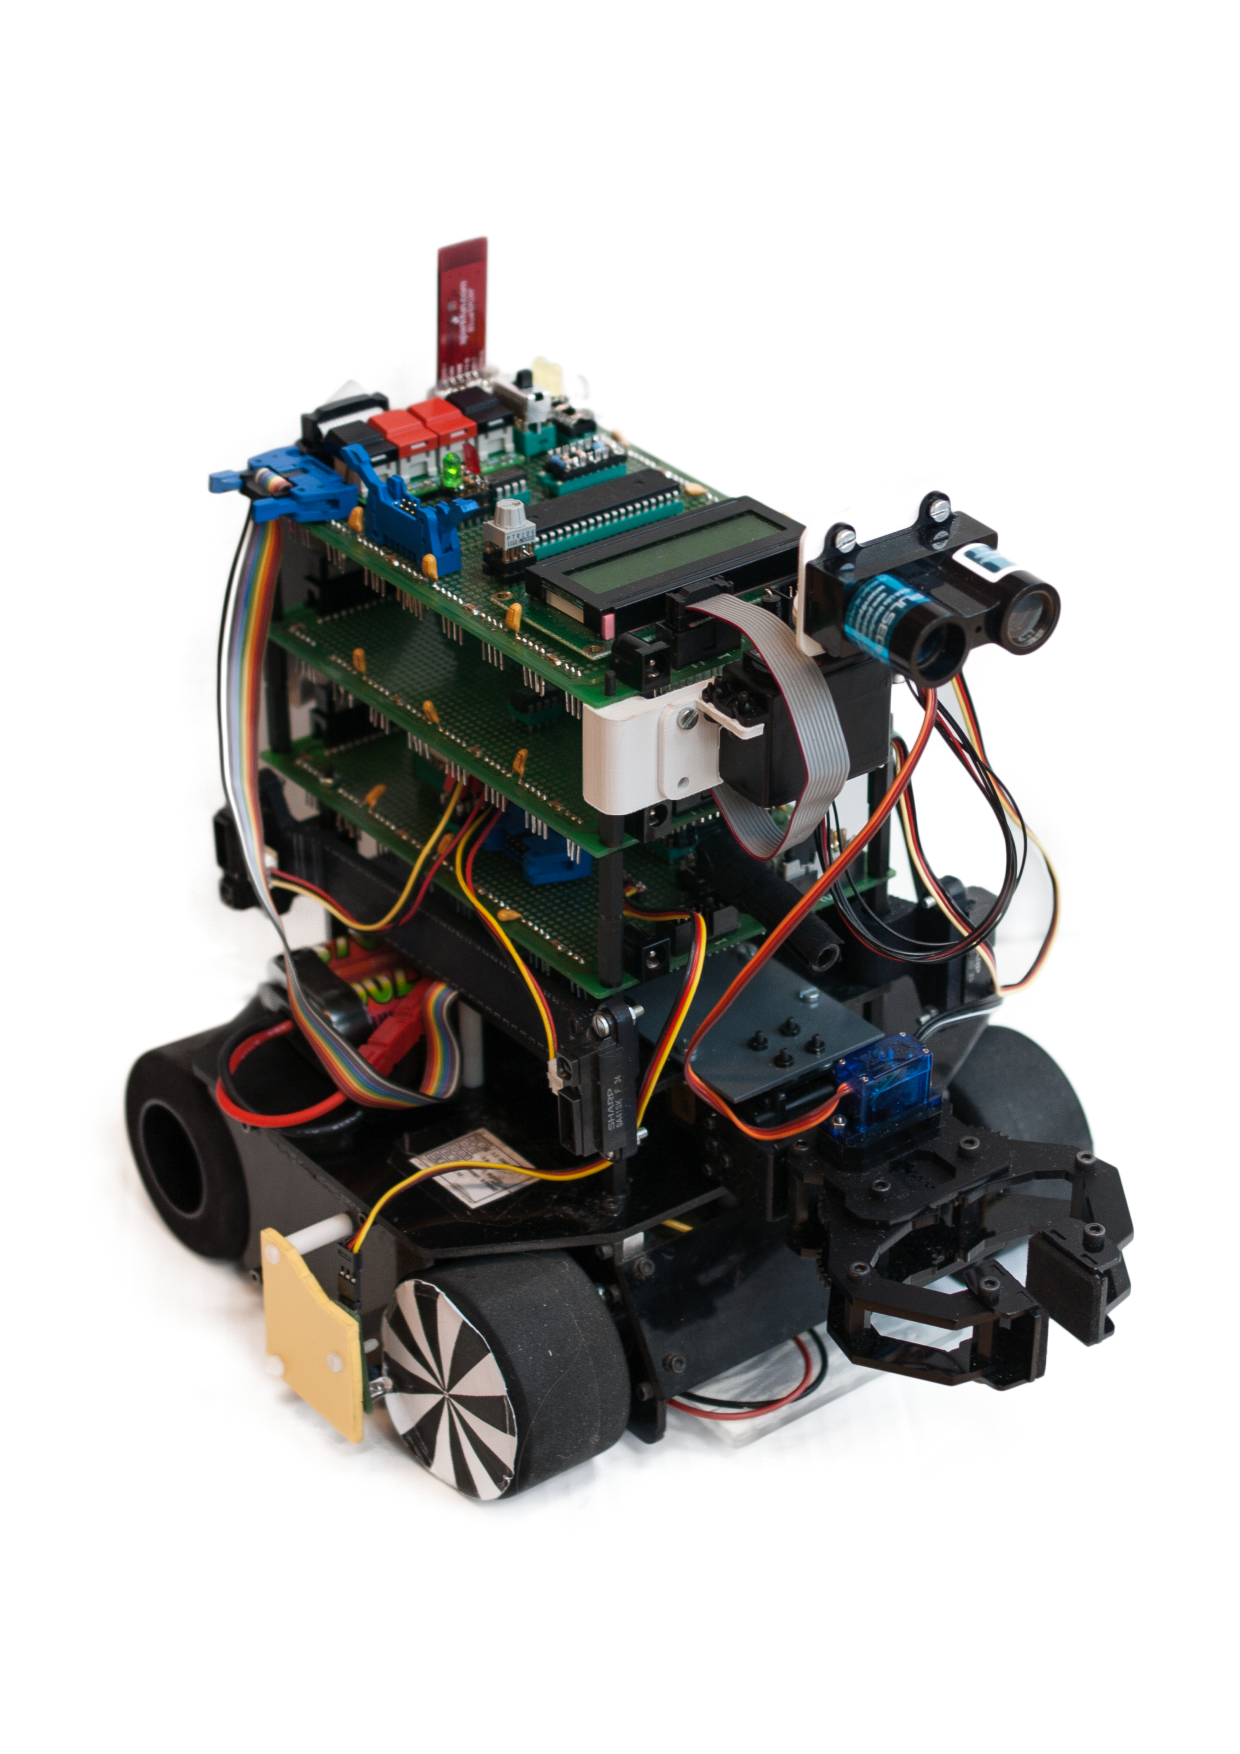
\includegraphics[width=0.9\textwidth]{images/RobotFront.pdf}
    \end{column}%
    \begin{column}{0.5\textwidth}
      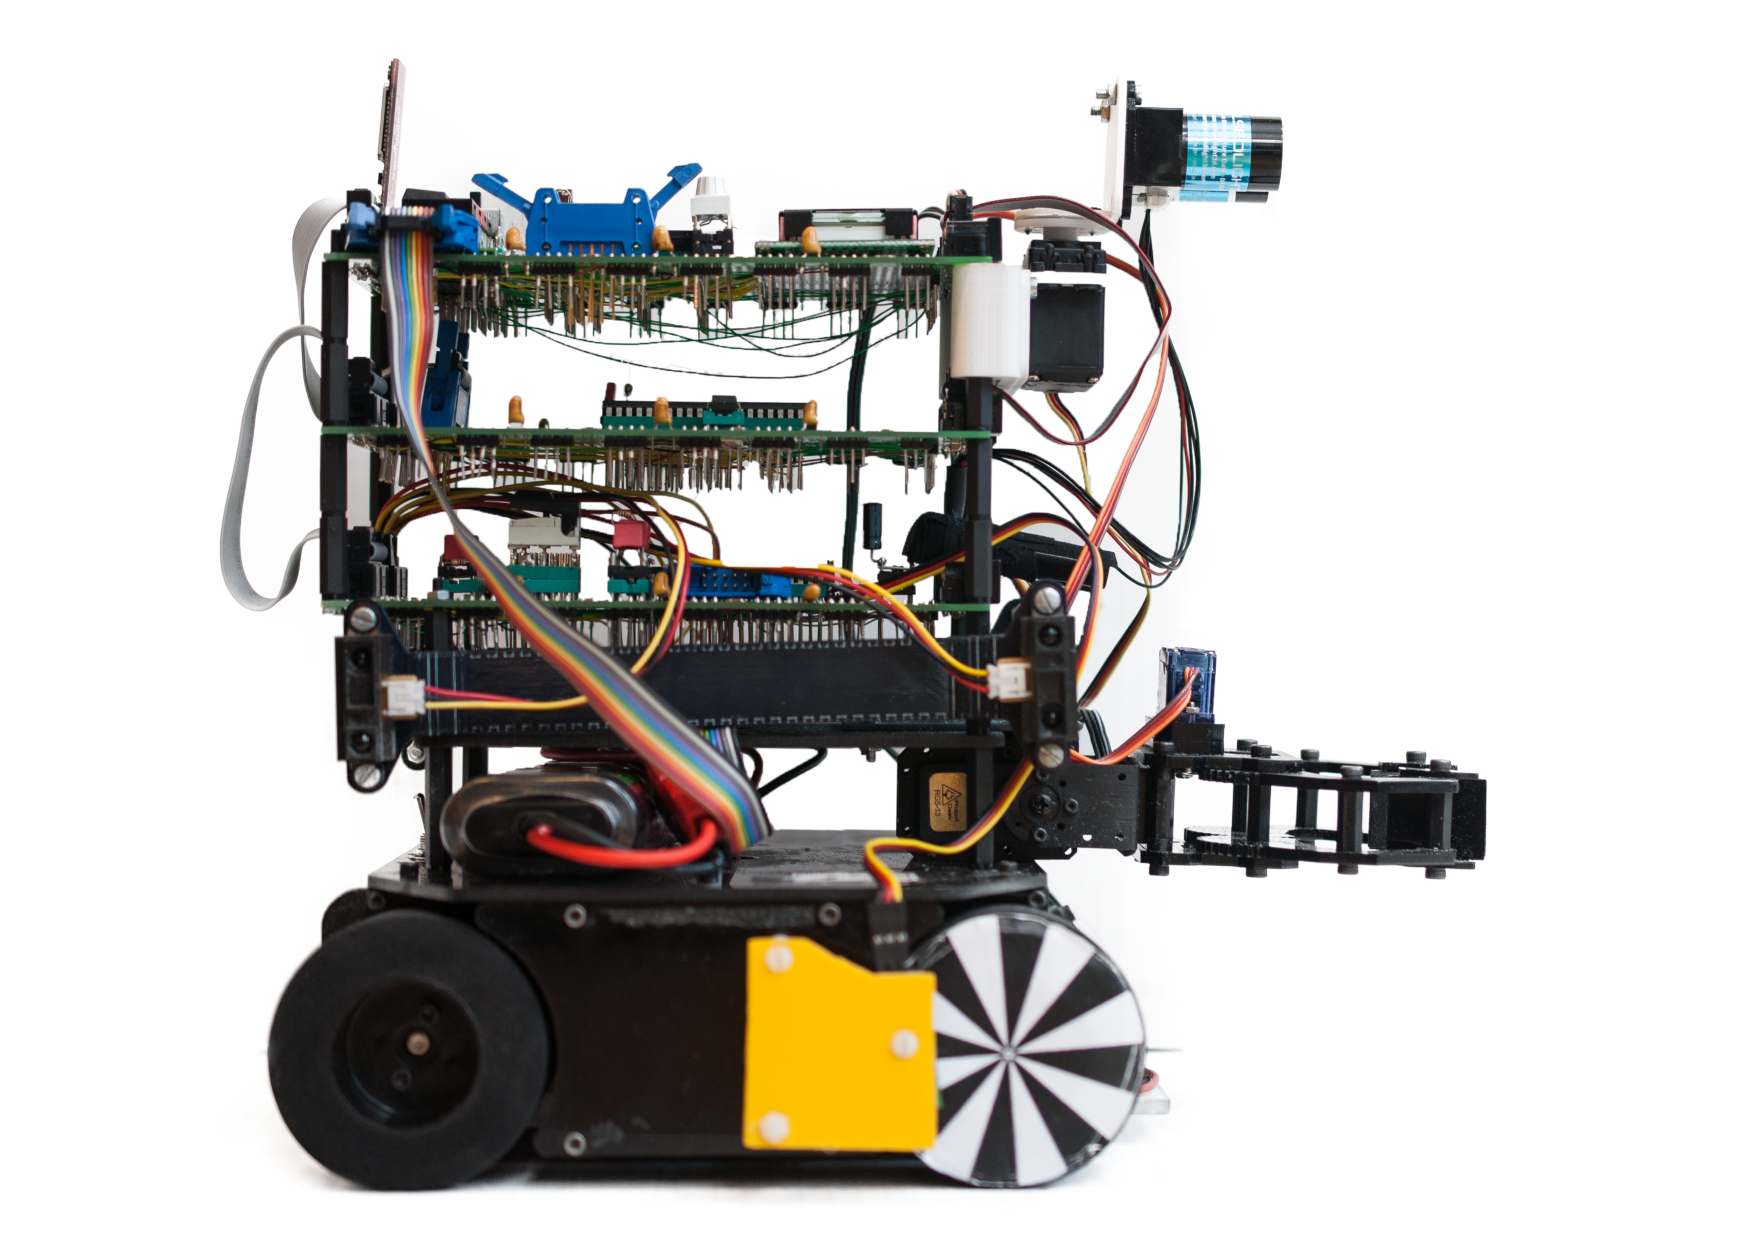
\includegraphics[width=\textwidth]{images/RobotSide.pdf}
    \end{column}
  \end{columns}
\end{frame}

\begin{frame}[fragile]{PigBot}
  \begin{itemize}
    \item[-] Undsättningsrobot på prototypnivå
\pause
    \item[-] Utforskar autonomt ett simulerat grottsystem
\pause
    \item[-] Kommunicerar kartdata till extern dator via Bluetooth\textsuperscript{\circledR}
\pause
    \item[-] Identifierar och undsätter en nödställd

  \end{itemize}
\end{frame}

\begin{frame}[fragile]{PigBot}
  \begin{columns}
     \documentclass{minimal}
\usepackage{tikz}
%\usetikzlibrary{calc,trees,positioning,arrows,chains,shapes.geometric,decorations.pathreplacing,decorations.pathmorphing,shapes,matrix,shapes.symbols}
\usetikzlibrary{positioning}
\usetikzlibrary{shapes}

\begin{document}
\begin{center}
\begin{tikzpicture}[scale=1]
\tikzset{every node/.style={inner sep=10pt, minimum width=3 cm}}
%\draw[help lines,step=5mm,gray!20] (-5,-10) grid (5,0);
\node[draw, fill=white] (Huvudmodul)  {\textbf{Huvudmodul}};
\node[draw,below left= of Huvudmodul] (Sensormodul) {\textbf{Sensormodul}};
\node[draw,below right = of Huvudmodul] (Styrenhet) {\textbf{Styrenhet}};
\node[draw, above = of Huvudmodul] (Datormodul) {\textbf{Datormodul}};
\node[ellipse,draw, right = of Datormodul] (Användare) {\textbf{Användare}};

\draw[->] (Huvudmodul) [out=300, in= 90] to (Styrenhet);
\draw[->] (Sensormodul) [out=90, in=240] to (Huvudmodul);
\draw[<->] (Huvudmodul) to (Datormodul);
\draw[<->] (Datormodul) to (Användare);
\end{tikzpicture}
\end{center}

\vspace{10em}

\begin{center}
\begin{tikzpicture}[scale=1]
\tikzset{every node/.style={inner sep=10pt, minimum width=3 cm}}
%\draw[help lines,step=5mm,gray!20] (-5,-10) grid (5,0);

\node[draw] (Sensormodul) {\textbf{Sensormodul}};
\node[above right = of Sensormodul,minimum width=0,inner sep=2pt] (Huvudmodul) {Huvudmodul};

\node[below left = of Sensormodul, minimum width = 0, inner sep = 2pt] (Sensor) {Sensorer};


\draw[->] (Sensor) [out=0,in=270] to node [sloped, midway, below] {spänningsnivåer} (Sensormodul);
\draw[->] (Sensormodul) [out=90,in=180] to node [sloped,midway, above] {enheter}  (Huvudmodul);

\end{tikzpicture}
\end{center}

\vspace{10em}

\begin{center}
\begin{tikzpicture}[scale=1]
\tikzset{every node/.style={inner sep=10pt, minimum width=3 cm}}
%\draw[help lines,step=5mm,gray!20] (-5,-10) grid (5,0);

\node[draw] (Styrmodul) {\textbf{Styrmodul}};
\node[above left = of Styrmodul,minimum width=0,inner sep=2pt] (Huvudmodul) {Huvudmodul};

\node[below right = of Styrmodul, minimum width = 0, inner sep = 2pt] (Motorer) {Motorer};
%\node[below left = of Styrmodul, minimum width = 0, inner sep= 2pt] (Gripklo) {Gripklo}


\draw[->] (Styrmodul) [out=270,in=180] to node [sloped, midway, below] {spänningsnivåer} (Motorer);
\draw[<-] (Sensormodul) [out=90,in=0] to node [sloped,midway, above] {kommandon}  (Huvudmodul);

\end{tikzpicture}
\end{center}

\vspace{10em}

\begin{center}
\begin{tikzpicture}[scale=1]
\tikzset{every node/.style={inner sep=10pt, minimum width=3 cm}}
%\draw[help lines,step=5mm,gray!20] (-5,-10) grid (5,0);

\node[draw] (Datormodul) {\textbf{Datormodul}};
\node[below = 10 em of Datormodul,minimum width=0,inner sep=2pt] (Huvudmodul) {Huvudmodul};
\node[right = of Datormodul, ellipse, draw] (Användare) {Användare};

%\node[below right = of Styrmodul, minimum width = 0, inner sep = 2pt] (Motorer) {Motorer};
%\node[below left = of Styrmodul, minimum width = 0, inner sep= 2pt] (Gripklo) {Gripklo}


\draw[->] (Datormodul) [out=30,in=150] to node [midway, above] {karta} (Användare);
\draw[<-] (Datormodul) [out=-30,in=210] to node [midway, below] {kommandon}  (Användare);

\draw[->] (Datormodul) [out=300,in=60] to node [near end, right] {kommandon} (Huvudmodul);
\draw[<-] (Datormodul) [out=240,in=120] to node [near end, left] {sensordata} (Huvudmodul);

\end{tikzpicture}
\end{center}


\end{document}
  \end{columns}

\end{frame}


\begin{frame}[fragile]{PigBot}
  \begin{itemize}
    \item[-] Tre stycken \Verb+ATmega1284p+
\pause
    \item[-] Åtta stycken sensorer
    \item[-] Osv\ldots
  \end{itemize}
\end{frame}

\end{document}



